\section{Results}\label{s:evaluation}
\subsection{Data Processing}
To process the data for analysis, we first eliminated potentially outlying trials. On Jatos we had a total of 99 submissions, but only 49 are finished experiments. First we excluded all experiments conducted from a browser smartphone based on the operating system logged by OpenSesame and on the window with less than 750 pixels. This resulted in 4 sessions being removed, reducing the number of trials from 2940 to 2700.
Since this experiment relies on sensory memory to an extent, we eliminate trials where the response time is unreasonably long - which could happen if the subject gets distracted for whatever reason - and trials where the response time is too short - which could happen if the subject accidentally clicks the response button without having time to think about the answer. To do this, the 1st and 99th percentiles of the response times where calculated, adjusted respectively by a factor of 1.5 in order to avoid discarding valid samples. This procedure identified 4 trials below the low cutoff of 243 ms and 16 trials above the high cutoff of 7828 ms. In order to keep the data paired, in the sense that each scene is presented once with a majority blue and majority red configuration, the other version of the outlying trial was removed as well, total of 40 trials removed. Finally, we removed another session where the subject entered an age of 169. Thus the clean data set consisted of 44 sessions with 2600 trials in total.

\subsection{General overview}
In Figure \ref{stats1} we can see the distributions of age, response times, gender and football experience level of the participants as well as favourite colours. 
\begin{figure}[h!]
    \hspace{-0.5cm} % Adjust this value to move the figure to your desired position
    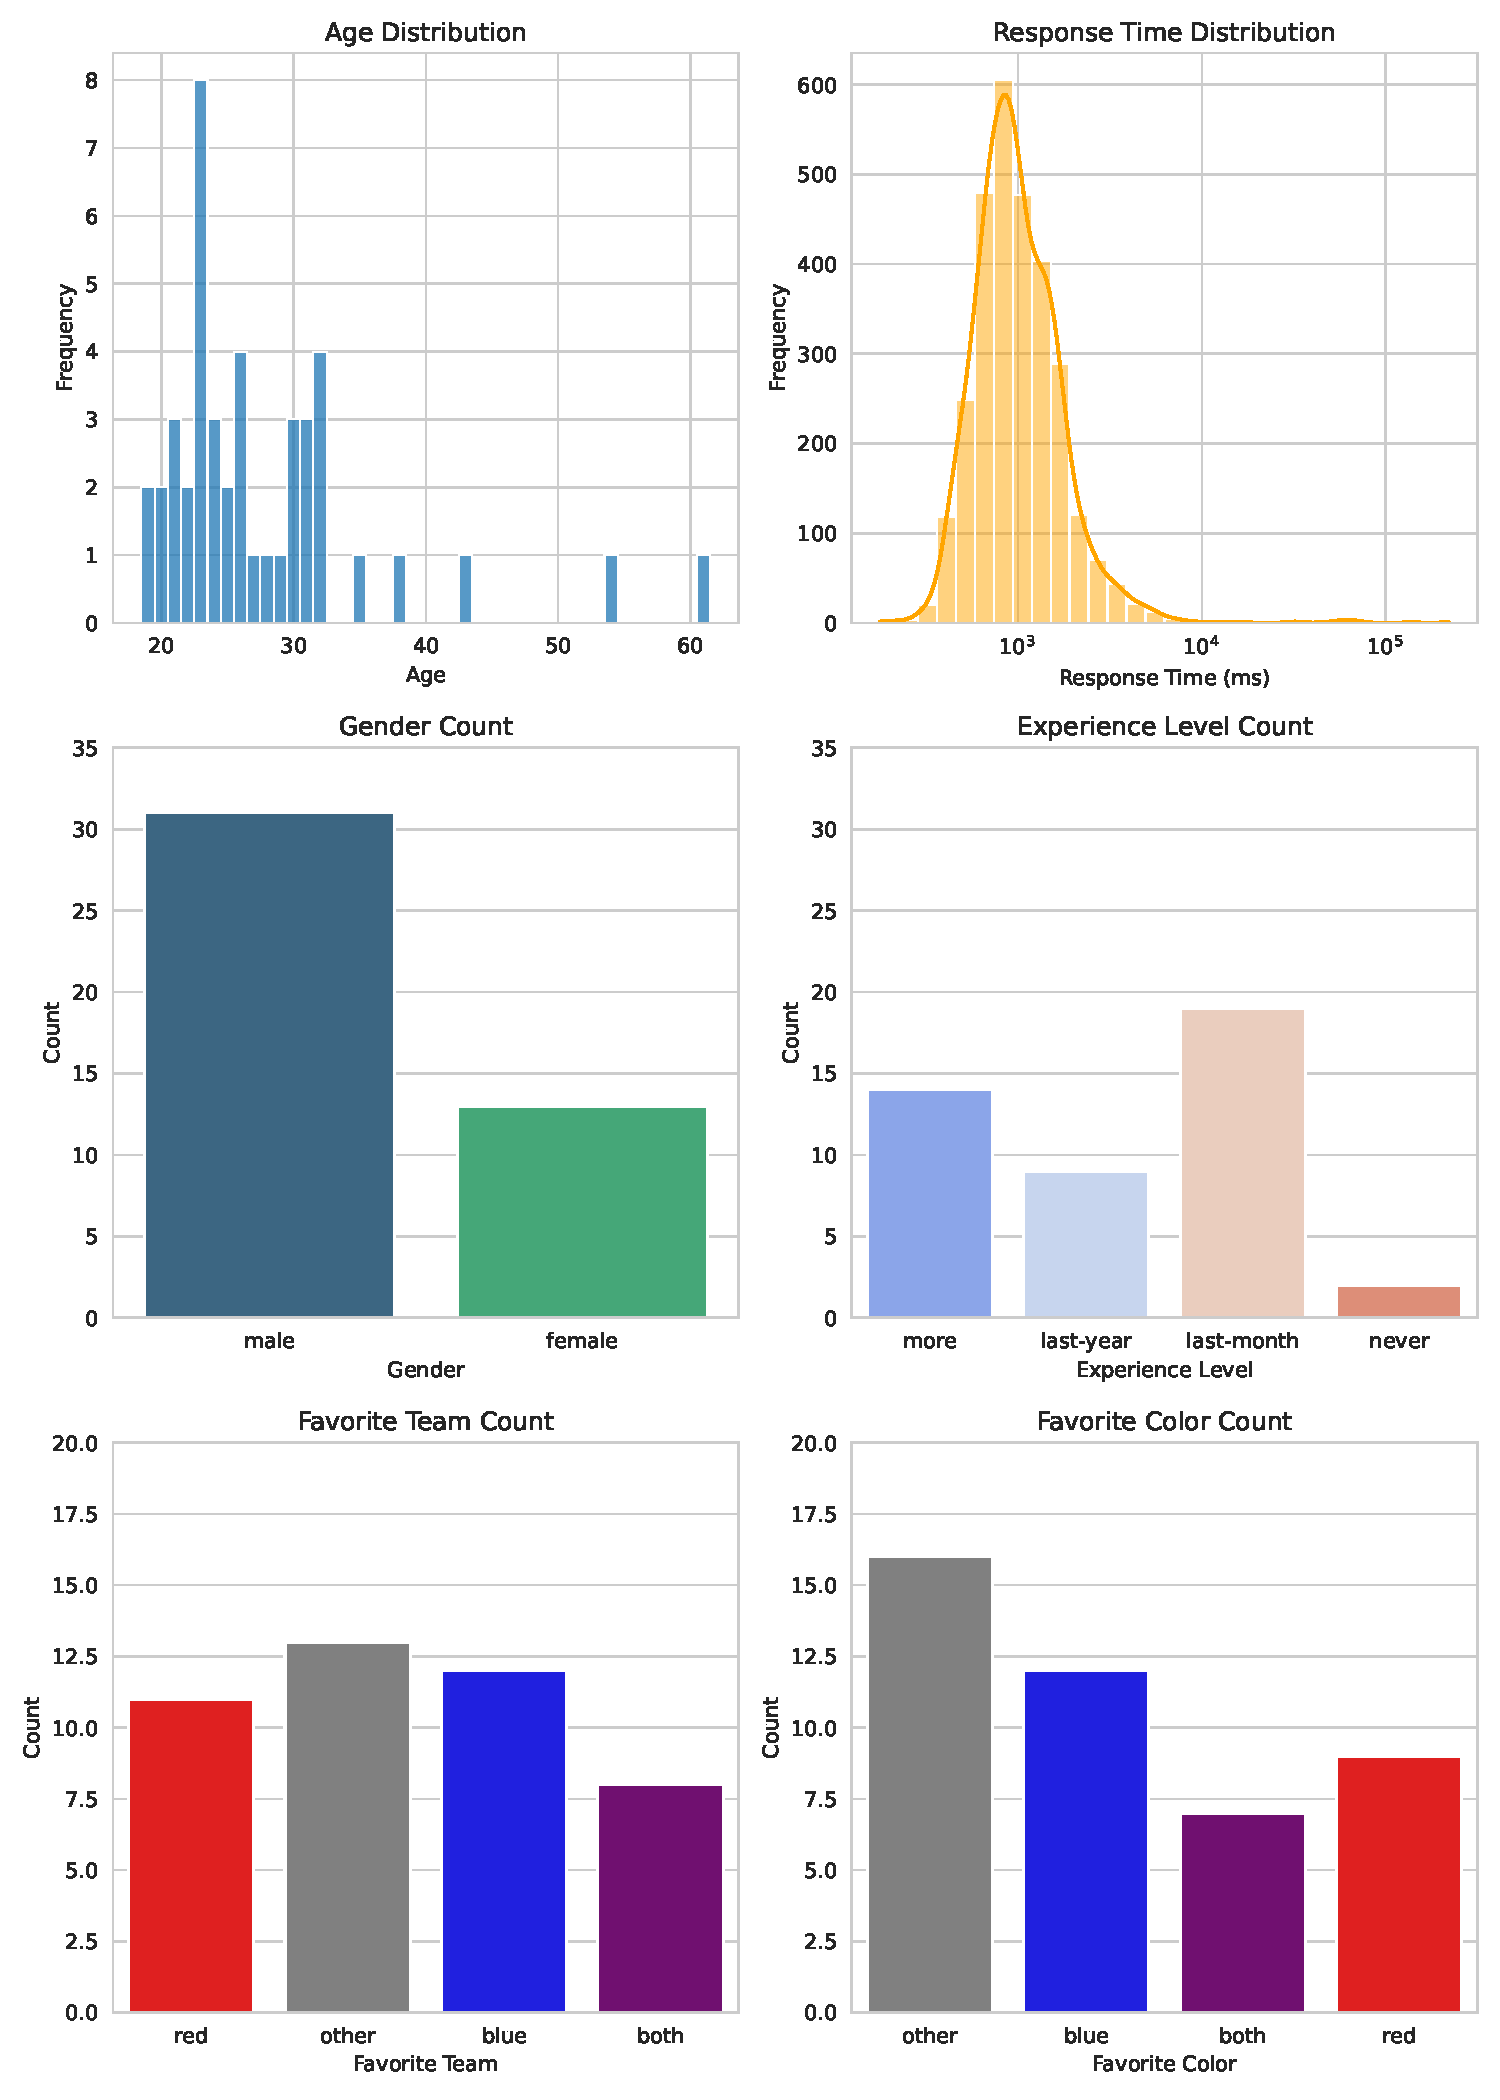
\includegraphics[width=\columnwidth]{vu-is-research-thesis/resources/demography.pdf}
   \caption{data set at a glance}
   \label{stats1}
\end{figure}
As is evident, the dataset currently skews towards younger male subjects, potentially making it more difficult to draw conclusions based on age or gender. 
% In Figure \ref{stats2}, we present an histogram of side with the most players, which serves as the correct answer (expected side) for each stimulus. We compare it them with participants' guesses, that favor the blue team more often.
% We also incorporate data on participants' favorite team colors and personal favorite colors, which we collected at the conclusion of the experiment. From the latter, it's evident that there's a minor inclination toward blue, although it's not as statistically significant as the imbalance in user responses.
\subsection{Findings}
The main research question is if the jersey colour of the majority team has an effect on accuracy. In order to investigate this question we examined the impact of various factors on accuracy. In the first row of figure \ref{stats2} it can be clearly observed that there are more trials where subjects thought that blue is the majority team compared to red, so accuracy for blue is higher. For reference, the top right plot depicts that the ground truth data is equally split between majority red and blue. 
\begin{figure}[h!]
    \hspace{-0.5cm} % Adjust this value to move the figure to your desired position
    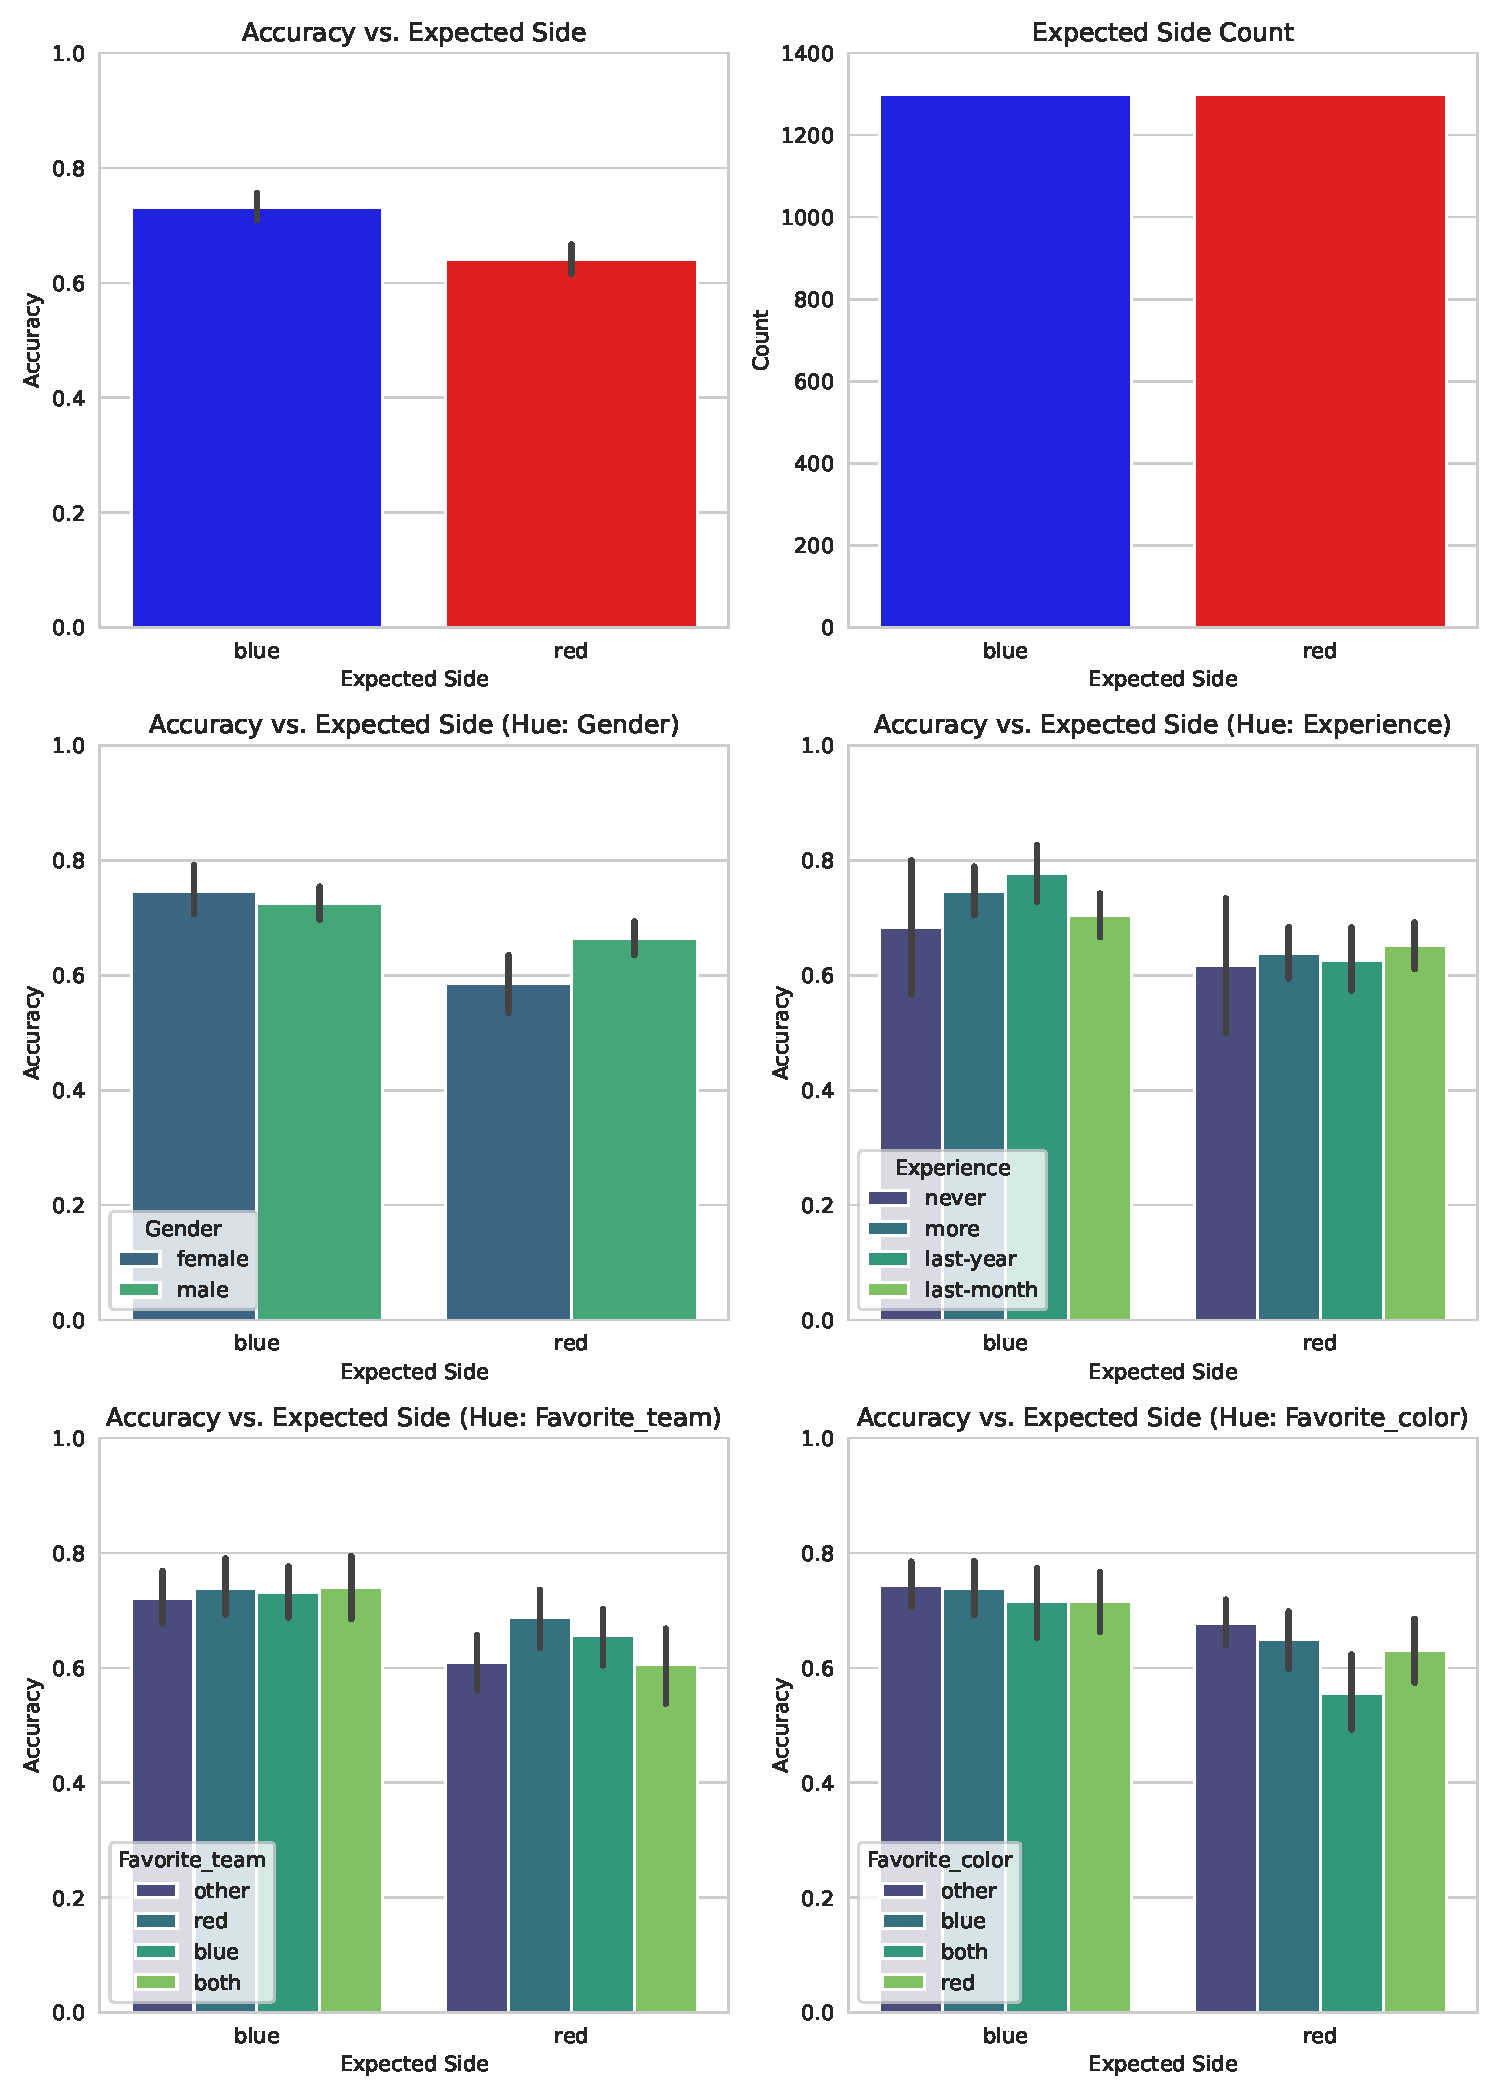
\includegraphics[width=\columnwidth]{vu-is-research-thesis/resources/accuracy_breakdown.pdf}
   \caption{accuracy breakdown}
   \label{stats2}
\end{figure}
In the next rows of figure \ref{stats2}, since the effect of expected side seems clear, the accuracy is additionally plotted by other factors. In the second row on the left the accuracy is additionally plotted by gender and on the right by experience. The by-gender breakdown seems to indicate that the effect is less pronounced for males since the difference in height for expected side blue and expected side red bars, is smaller for males. The by-experience plot indicates that the effect is least pronounced for subjects who played or watched football during the last month and the effect is much more pronounced for subject doing this one year ago or more. For the by-favourite-team and by-favourite colour plots it's not immediately clear if there is a difference given the long error-bars, the most noticeable effect perhaps being that the effect is less pronounced if the favourite team is red. The plot is just indicative of possible effects, next we will present the results of statistical tests aimed at quantifying the significance and magnitude of the effects.

\subsubsection{Models and test}

Before proceeding with more complex models, we first ran statistical tests on the contingency table of expected colour versus correctness of response. The Chi-Square test and the proportion test are applicable, and result in significant p-values (8e-7). Since the data is paired, McNemar's test is the more valid options and because the statistical power of this test is higher, it results in an even more significant p-value of 1e-8. 

Next a generalized linear model with a logistic link function is fit where the dependent variable is the $is_correct$ variable and the independent variable is only the expected (majority) side. Table \ref{table:glm_results} shows that even ignoring all other factors, the $expected\_side$ is a significant predictor of the $correct\_response$, and specifically, when the expected side is "red", the likelihood of a correct response decreases, more specifically, log odds of a correct response decrease by approximately 0.46. Given that $\operatorname{logit}\left(P_{\text {red }}\right)=\beta_0+\beta_1 \times 1=1.0024-0.4237$ the expected probability of a correct response when the majority side is red is $P_{\text {red }}=\frac{e^{\operatorname{logit}\left(P_{\text {red }}\right)}}{1+e^{\operatorname{logit}\left(P_{\text {red }}\right)}}=0.641$ and similarly $P_{\text {blue }}=0.732$. The statistical tests and the basic logistic model show beyond with great statistical certainty that subjects are biased towards blue. Next, similar to the rows of figure \ref{stats2}, several models will be presented, checking for more subtle effects.

\begin{table}[h]
    \centering
    \caption{GLM results for the effect of team color on correct response.}
    \begin{tabular}{lcccc}
        \hline
        Coeff. & Est. & Std. Error & z value & Pr(>|z|) \\
        \hline
        Intercept & 1.002 & 0.063 & 16.02 & $< 2 \times 10^{-16}$ *** \\
        expected\_side=red & -0.424 & 0.086 & -4.97 & $6.6 \times 10^{-7}$ *** \\
        \hline
    \end{tabular}
    \label{table:glm_results}
\end{table}

The basic logistic model above ignores random effects, so we ran a linear mixed-effect model (LMM) with $expected\_side$ as fixed effects and by-subject and by-scene random intercepts for the $expected\_side$ variable and we also check whether adding a random slope as well improves the model. By doing an Anova test we find that adding a random slopes doesn't significantly improve the model. Table \ref{table:glmer_results} contains the model fitted on 2600 observations where there are 44 groups for subject\_id and 30 groups for scene\_id variables.

\begin{table}[h]
    \centering
    \caption{Mixed-effects model results for the effect of team color on correct response, accounting for random effects of subject and scene.}
    \begin{tabular}{lcccc}
        \hline
        Coeff. & Est. & Std. Error & z value & Pr(>|z|) \\
        \hline
        Intercept & 1.185 & 0.177 & 6.69 & $2.2 \times 10^{-11}$ *** \\
        expected\_side=red & -0.491 & 0.091 & -5.37 & $7.9 \times 10^{-8}$ *** \\
        \hline
    \end{tabular}
    \label{table:glmer_results}
\end{table}

The variance for the random effect of subject (\textit{subject\_id}) is 0.252, indicating a moderate degree of variability in correct responses across subjects. The variance for the random effect of scene (\textit{scene\_id}) is 0.621, indicating a higher degree of variability in correct responses across different scenes. We note that considering the random effects the significance of the difference between the log odds of correct responses for red and blue majority trials becomes more significant by an order of magnitude.

Table \ref{table:glmer_results_interaction} summarises the model which considers genders as an additional fixed effect, in interaction with expected side. This model quantifies the difference depicted in figure \ref{stats2} middle left. This model, shows that while gender by itself is not a good predictor of accuracy, its effect becomes significant as an interaction with the expected side. In other words, the effect of expected side on accuracy is not the same for males and females. More specifically, the expected log odds of a correct answer for a female subject is 1.253 for a majority blue sitmulus but odds decrease significantly by 0.838 when the expected side is red to 0.415. The expected log odds for a male when majority blue is 0.098 lower than a female, but this difference is not significant, but when the majority is red, the expected log odds of correct response rise to 1.253 - 0.098 + 0.410 = 1.655.
\begin{table}[h]
    \centering
    \caption{GLMM results for the effect of team color and gender on correct response, with random effects of subject and scene.}
    \begin{tabular}{lcccc}
        \hline
        Coeff. & Est. & Std. Error & z value & Pr(>|z|) \\
        \hline
        Intercept & 1.253 & 0.236 & 5.31 & $1.1 \times 10^{-7}$ *** \\
        e\_s=red & -0.838 & 0.166 & -5.03 & $4.8 \times 10^{-7}$ *** \\
        gndr=male & -0.098 & 0.221 & -0.44 & 0.657 \\
        e\_s=red:gndr=male & 0.410 & 0.199 & 2.51 & 0.012 * \\
        \hline
    \end{tabular}
    \label{table:glmer_results_interaction}
\end{table}
Finally, we check favourite colour, favourite team and experience as covariates in interaction with expected side but do not find statistically significant effects. Some interesting qualitatitive observations can be made based on these figures. While the response time distributions are basically identical for blue/red expected sides which is interesting because it indicates that the duration of the cognitive mechanisms which leads to the estimation bias is not itself affected by the majority colour. A subtle difference in the distributions can be observed for correct and incorrect responses, where incorrect responses tend to have more shorter response times and more longer response times. Perhaps most intriguingly, the RT distribution is significantly different between males and females, where female subjects not only tend to respond slower on average, but the response time is also bimodal. 

\subsubsection{Response times}
In addition to the accuracy, a secondary investigation can be performed on the response times. In particular figure \ref{stats3} depicts the response times for correct/incorrect responses, male/female subjects and blue/red expected sides.
\begin{figure}[h!]
    \hspace{-0.5cm} % Adjust this value to move the figure to your desired position
    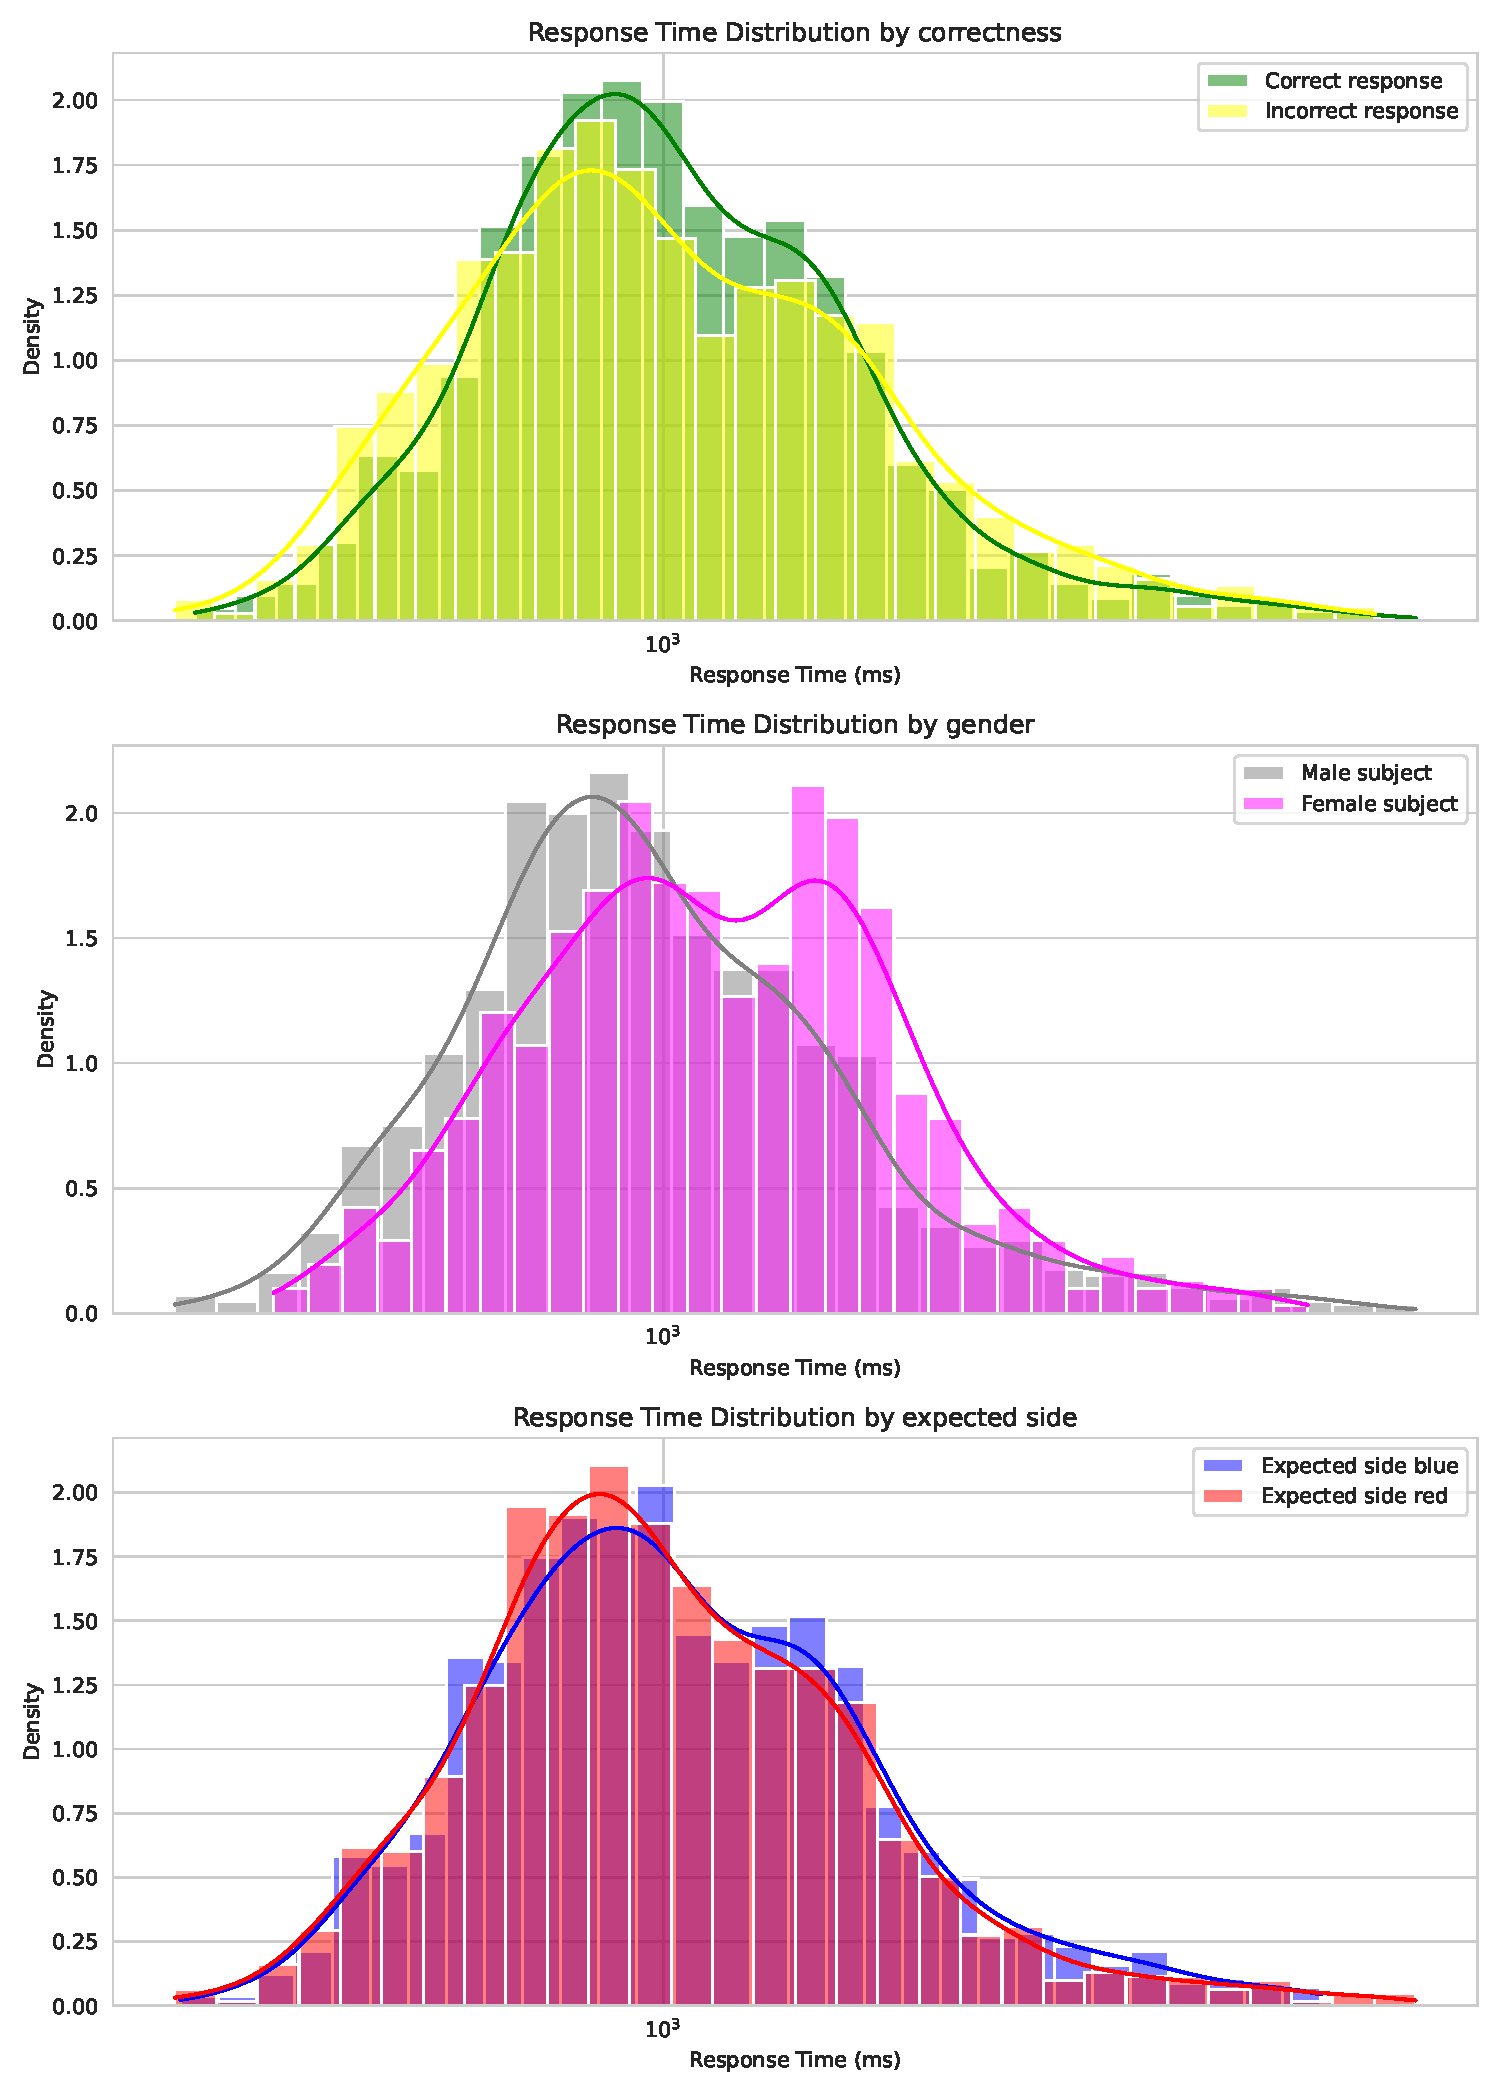
\includegraphics[width=\columnwidth]{vu-is-research-thesis/resources/response_times.pdf}
   \caption{response time distributions}
   \label{stats3}
\end{figure}
While the response time distributions reveal interesting avenues of further investigation, given the current data, it is not immediately clear how the response time data can be interpreted to explain the color salience research question.